\begin{frame}
\frametitle{Parallélisation MPI}
\vfill
Pour compenser la faible quantité de mémoire GPU et accélérer les calculs :
\begin{itemize}
\item Exécution multi-GPU via MPI ;
\item Chaque GPU est associé à un processus MPI (mémoire distribuée) ;
\item Partitionnement équilibré du maillage ;
\item Communications MPI au niveau des interfaces entre zones.
\end{itemize}
\vfill
\begin{figure}
	\centering\small
		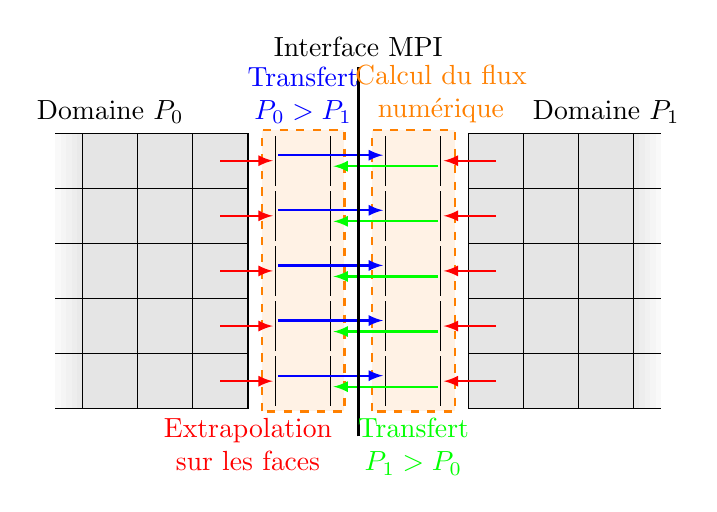
\begin{tikzpicture}[scale=0.7]
		\draw[thick,dashed,orange,fill=orange!10] (4.25,-0.05) rectangle (5.75,5.05);
		\draw[thick,dashed,orange,fill=orange!10] (6.25,-0.05) rectangle (7.75,5.05);
		
		\fill[gray!20] (1,0) rectangle (4,5);
		\fill[gray!17] (0.9,0) rectangle (1.0,5);
		\fill[gray!14] (0.8,0) rectangle (0.9,5);
		\fill[gray!11] (0.7,0) rectangle (0.8,5);
		\fill[gray!08] (0.6,0) rectangle (0.7,5);
		\fill[gray!05] (0.5,0) rectangle (0.6,5);

		\fill[gray!20] (8,0) rectangle (11,5);
		\fill[gray!17] (11.0,0) rectangle (11.1,5);
		\fill[gray!14] (11.1,0) rectangle (11.2,5);
		\fill[gray!11] (11.2,0) rectangle (11.3,5);
		\fill[gray!08] (11.3,0) rectangle (11.4,5);
		\fill[gray!05] (11.4,0) rectangle (11.5,5);

		\foreach \i in {0,1,2,3,4,5} {
			\draw[-] (0.5,\i) -- (4,\i);
			\draw[-] (8,\i) -- (11.5,\i);
		}
		\foreach \i in {1,2,3,4,8,9,10,11} {
			\draw[-] (\i,0) -- (\i,5);
		}
		\foreach \i in {4.5,5.5,6.5,7.5} {
			\draw[-] (\i,0.05) -- (\i,0.95);
			\draw[-] (\i,1.05) -- (\i,1.95);
			\draw[-] (\i,2.05) -- (\i,2.95);
			\draw[-] (\i,3.05) -- (\i,3.95);
			\draw[-] (\i,4.05) -- (\i,4.95);
		}
		\foreach \i in {0.5,1.5,2.5,3.5,4.5} {
			\draw[arrows={-latex},thick,red] (3.5,\i) -- (4.45,\i);
			\draw[arrows={-latex},thick,red] (8.5,\i) -- (7.55,\i);
		}
		\foreach \i in {0.6,1.6,2.6,3.6,4.6} {
			\draw[arrows={-latex},thick,blue] (4.55,\i) -- (6.45,\i);
		}
		\foreach \i in {0.4,1.4,2.4,3.4,4.4} {
			\draw[arrows={-latex},thick,green] (7.45,\i) -- (5.55,\i);
		}
		
		\draw[very thick] (6,-0.5) -- (6,6.2) node[above] {Interface MPI};
		\draw (1.5,5) node[above] {Domaine $P_0$};
		\draw (10.5,5) node[above] {Domaine $P_1$};
		\draw (4,0) node[below,red,align=center] {Extrapolation\\sur les faces};
		\draw (5,5) node[above,blue,align=center] {Transfert\\$P_0 > P_1$};
		\draw (7,0) node[below,green,align=center] {Transfert\\$P_1 > P_0$};
		\draw (7.5,5) node[above,orange,align=center] {Calcul du flux\\numérique};
		
		\end{tikzpicture}
\end{figure}
\vfill
\end{frame}

